\section{Uppgift 3}\label{sec:uppg03}

\subsection{Instruktioner}
\begin{Verbatim}[fontsize=\small]
I denna uppgift ska du använda dig av klassen Person som du skrev i laboration
3, *utan* att göra några ändringar i den. Skriv en till klass Student som ärver
klassen Person (Student blir alltså en subklass till Person). I klassen Student
ska du ha dessa instansvariabler:

kurs (String)
betyg (char)
skola (String)

I klassen Student ska du ha följande metoder:

- ändraKurs, ändrar kurs enligt parameterns värde.
- ändraBetyg, ändrar betyg enligt parameterns värde.
- ändraSkola, ändrar skola enligt parameterns värde.
- hämtaKurs, returnerar kurs.
- hämtaBetyg, returnerar betyg.
- hämtaSkola, returnerar skola.
- toString, en metod som i en snyggt formaterad sträng returnerar ett
  Student-objekts *samtliga* data, även indirekt "ärvda" data från klassen
  Person. Metoden anropas genom att skriva objektets (referensens) namn.

Och naturligtvis ska du ha med en konstruktor, där du ska initiera alla
instansvariabler inkl de som ligger i superklassen Person.

Skriv slutligen en testklass där du skapar ett Person-objekt och ett
Student-objekt.  Testa först alla metoder som går att anropa på Person-objektet
och testa sedan alla metoder som går att anropa på Student-objektet.
\end{Verbatim}


\subsection{Källkod}
\subsubsection{Lab4Uppg03.java}
\javacode{src/Lab4Uppg03.java}
\caption{Lab4Uppg03.java}
\label{src:uppg03}

\subsubsection{Student.java}
\javacode{src/Student.java}
\caption{Student.java}
\label{src:student}

\subsubsection{Person.java}
\javacode{src/Person.java}
\caption{Person.java}
\label{src:person}

% Screenshots med Bash, terminalfönsterstorlek 90x40
\subsection{Skärmdump}
Se Figur~\ref{fig:uppg03-screenshot} för skärmdump på körning av koden i
Sektion~\ref{src:uppg03}, Sektion~\ref{src:student} och
Sektion~\ref{src:person}.

\begin{figure}[htbp]
\centering
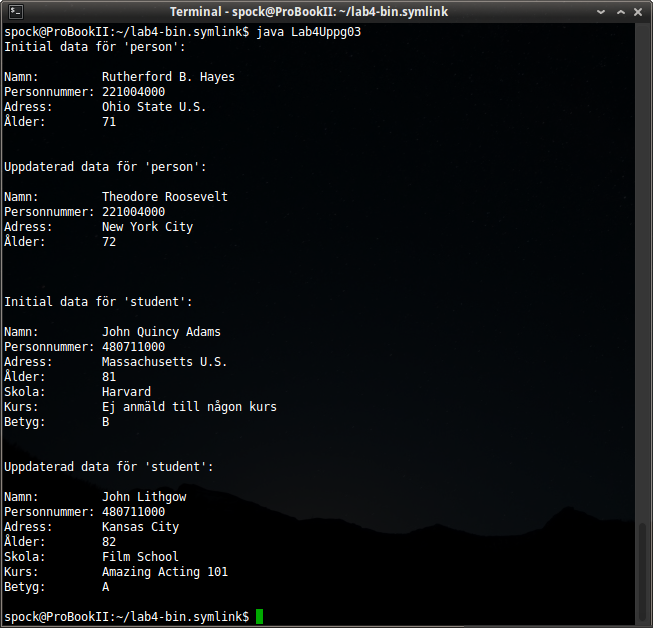
\includegraphics[width=\linewidth]{img/03.png}
\caption{Körning av koden till Uppgift~\ref{sec:uppg03}}
\label{fig:uppg03-screenshot}
\end{figure}

